\chapter{Configuring xymon Monitoring}
\section{Configuring xymon Monitoring}


 The xymon configuration is kept in the files in the ~/server/etc/
 directory. If you look at this directory, you will see these files:

\begin{itemize}
\item \motoserverconfig{bb-hosts} is the one you will change the most. This file contains
  a list of all the hosts you are monitoring, including information
  such as their IP-address, what network services you are monitoring
  on the host, what URL's you are checking, what subpage in the xymon
  web-pages this host is shown on etc. The name of the file -
  ``bb-hosts'' - was chosen so it is compatible with the Big Brother
  system which uses the same filename and file format.

\item \motoserverconfig{xymon-clients.cfg} is the configuration file for data reported
  by the xymon clients installed on the hosts you are
  monitoring. This defines the color of the cpu-, disk-, memory- and
  procs-columns, based on the information that is sent to xymon by
  the clients.

\item \motoserverconfig{xymon-alerts.cfg} holds the alerting configuration. In this
  file, you setup the rules for sending out alerts about services
  going down: Who gets the alert, how is it sent, how often, whether
  to send alerts 24x7 or only between 10 AM and 4 PM on weekdays etc.

\item \motoserverconfig{xymonserver.cfg} is the configuration file for the xymon
  server. This file defines a lot of environment variables that are
  made available to all of the xymon programs when they run. Some
  environment variables that are defined in the Big Brother system are
  also setup by xymon, so that Big Brother extension scripts will
  work. 

The initial configuration of xymonserver.cfg is setup by the
configure script when you install xymon, and in most cases you will
not need to change it.

\item \motoserverconfig{xymonlaunch.cfg} is the configuration file for the hobbitlaunch
  tool. xymonlaunch is the master program in xymon, it is the only
  program you start to run the xymon server. xymonlaunch reads the
  xymonlaunch.cfg file, and starts the programs listed here to run
  the server. Some of the programs may run as daemons, some of the
  programs may run at regular intervals. If you want to use some of
  the advanced options for the bbgen or bbtest-net programs, you
  change the xymonlaunch.cfg file to add these options to the
  commandline.

\item \motoserverconfig{xymongraph.cfg} is a configuration file for
  the xymongraph  CGI. It defines how the graphs are generated from
  the data in the  RRD files.



\item bb-services is a configuration file for the bbtest-net
  program. It defines how network services are checked.


\end{itemize}

\section{Setting up monitoring of hosts}


 The bb-hosts file defines which hosts xymon monitors. When you
 install xymon, a simple configuration is setup that just lists the
 xymon server: 

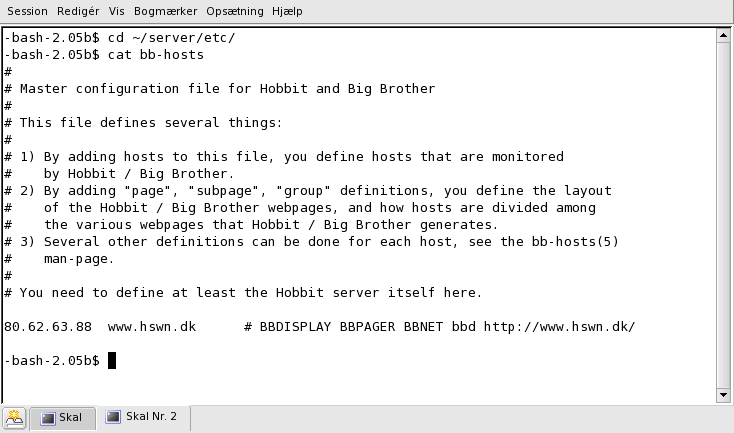
\includegraphics[scale=0.5]{./xymon-bbhosts.png} 


 There are a few things to notice here:
\begin{itemize}
\item Lines that begin with a \emph{\#}
 are comments.
\item Each host you monitor is on a line by itself, with the
  IP-address and the hostname of the host.

\item You can add extra tags to each host definition, by putting in a
  \#-mark and then some keywords. These keywords define how xymon
  handles the host.



\end{itemize}


 The bb-hosts file shown in the example has only one host defined: \emph{www.hswn.dk}
 which is the server running xymon. There are a few extra keywords thrown in:

\begin{itemize}
\item \emph{BBDISPLAY, BBPAGER, BBNET} are compatibility settings for
  extensions written for Big Brother. xymon doesn't use these, but
  puts them in the bb-hosts file to avoid problems if you mix xymon
  and Big Brother modules.

\item \emph{bbd}
 is the name of a \emph{network test}. This keyword causes the xymon
 network-tester bbtest-net to check if the bbd network service is
 running on this host, and send a status report to the xymon server
 with the information about this service. So you'll get a (hopefully!)
 green icon on the xymon webpage for this host, showing the status of
 the bbd network service. 

 Network services are defined in the \emph{bb-services} file, so this
 file must have an entry for bbd defining what TCP port to check, and
 possibly also what data to send to the service and what to expect as
 a response.

\item \emph{\url{http://www.hswn.dk/}}
 is a URL, obviously. This also triggers a network test, the xymon
 network tester will try to request this URL, and send in a status
 report showing if the URL was accessible or not.


\end{itemize}


 By default, xymon will always check if the host is up and running by
 trying to ``ping'' it. This results in a \emph{conn} column on the
 xymon webpage for this host, showing if the ping-test succeeded. If
 you have a host that does not respond to ping - e.g. because there is
 a firewall that filters out such requests - then you can disable the
 ping-test by putting a ``noconn'' keyword on the line in bb-hosts.



 As you can see, the syntax is pretty straight-forward. Need to
 monitor an extra URL for this server ? Just add the URL to the
 line. Need to check if ssh (Secure Shell) is running ? Just add
 \emph{ssh}

 to the line. The full set of keywords you can use is described in the
 bb-hosts man-page. Many of the keywords relate to the way xymon
 displays the information about the host on the web-pages, other
 keywords deal with how the uptime percentage is calculated for
 availability reports, and some keywords - like the \emph{bbd} and
 \emph{\url{http://...}} mentioned above - describe the network
 services that are tested for this host.

\subsubsection{Monitoring network services}


 As shown in the example above, adding a network test for a host is as
 simple as putting the right keyword into the bb-hosts file. The
 default set of network tests configured in xymon 4.0 is as follows:

\begin{table} \centering \caption{Monitored Network Services} \label{Monitored_Network_Services}
\begin{tabular}{l|l}
conn & Simple ping test. Enabled by default, you can disable it by putting ``noconn'' into bb-hosts.\\
http & Web-server test. Enter the URL to request from the webserver. \\
ftp & FTP server test. \\
ssh & SSH (Secure Shell) server test. Supports ssh1 and ssh2. \\
telnet & Telnet server test. \\
smtp & SMTP (Mail server) test.\\ 
pop3 & POP-3 test. \\
imap & IMAP test. IMAP version 2 and 4 are supported, for version 3 use ``imap3''. \\
nntp & NNTP (News) server test. \\
ldap & LDAP (Directory server) test. Enter the full LDAP URI if xymon is configured with LDAP support. \\
rsync & rsync server test. \\
bbd & Big Brother daemon test. Also works with the xymon network daemon. \\
clamd & CLAM anti-virus daemon test. \\
spamd & SpamAssassin anti-spam daemon test. \\
oratns & Oracle TNS listener test. Will attempt to do an oratns ``ping''. \\
qmtp & QMTP server test. For qmail's qmtpd service. \\
qmqp & QMQP server test. For qmail's qmqpd service.
\end{tabular}

\end{table}

 If xymon is built with OpenSSL support, the following SSL-enabled services can also be checked:

\begin{table} \centering \caption{Monitored Network Services with SSL enabled} \label{Monitored_Network_Services_SSL}
\begin{tabular}{l|l}
https & Web-server test. Enter the URL to request from the webserver.\\ 
ftps & Secure FTP server test. \\
telnets & Secure Telnet server test. \\
smtps & Secure SMTP server test. \\
pop3s & Secure POP-3 server test. \\
imaps & Secure IMAP server test. \\
nntps & Secure NNTP (News) server test. \\
ldaps & Secure LDAP (Directory) server test.
\end{tabular}

\end{table}

Enter the full LDAP URIif xymon is configured with LDAP support. Note that this is only
possible when xymon is built with the OpenLDAP v2.x client library,
and only for LDAP servers that support LDAP version 3 and the
``starttls'' command. LDAP server that use the older non-standard
method of tunnelling LDAP through SSL on port 636 will not work.





 There are a few network tests that xymon can run for you, by using
 external programs. This is not a very effective way of testing, so it
 is only done this way for a few very specialised tests:


\begin{table} \centering \caption{Other Monitored Network Services} \label{Other_Monitored_Network_Services}
\begin{tabular}{l|l}
ntp & NTP (Network Time protocol) server test, using the ``ntpdate'' command. \\
rpc & RPC service test. This queries the \emph{portmapper} service on
the server, using the ``rpcinfo'' command. See the
\textbf{bb-hosts(5)} man-page for details on how to test for specific
RPC services.

\end{tabular}
\end{table}

\subsubsection{Monitoring host-specific data with clients}


 You can install a client on each of the hosts you monitor, to check host-specific data such as CPU utilisation, disk usage, if certain processes and services are running etc. xymon includes clients for most Unix-like operating systems. A client for Windows is planned but the programming has not yet started.


 First, make sure you have installed the xymon client on all of the hosts you want to monitor, and you have these hosts listed in your bb-hosts file. The Xymon client will pick up the hostname of the box it is running on automatically, but it is not uncommon for the name it finds to be different from what you've put into bb-hosts. So if you know that the client is running but no data appears, check that the hostname used by the Hobbit client is the one you expect. See this FAQ item for details.


 With the xymon client running and reporting data into Xymon, you should see the cpu-, disk-, memory- and procs-columns appear. The color of these status columns is determined by settings in the  xymon-clients.cfg configuration file. Here is an example of how to setup a host:


 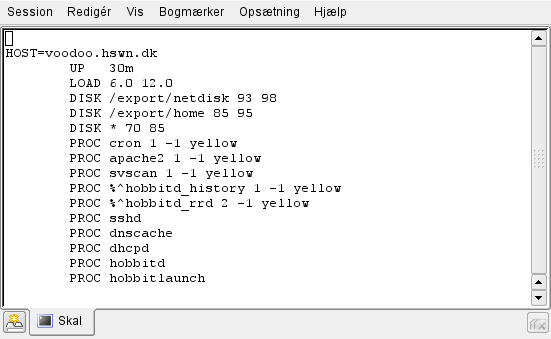
\includegraphics[scale=0.5]{./xymon-clients.png} 


 As you can see, there's first a definition of what hosts the following criteria applies to. Here, it is only a single host: voodoo.hswn.dk - but you can use various filters on hostnames, pagenames and time of day to determine what the thresholds should be for each of the criteria monitored with the client data. The xymon-clients.cfg man-page describes this in detail.


 After the host filter comes the criteria used to determine the color of each of the status columns.


\begin{tabular}{l|l}
UP & Sets the \textbf{cpu}  column color, based on how long the host has been up. After the UP keyword you put two time limits: The first one (30m in the example) defines how long after a reboot the cpu column is yellow. The second (optional) value causes the cpu column to go yellow after the host has been up for this long - it may be useful, if you need to reboot your servers regularly.  \\
LOAD & Sets the \textbf{cpu} \\
 column color, based on how much load is on the system. After the LOAD
 keyword you put two limits: The first number is the limit where the
 cpu column goes yellow; the second is the limit where the cpu column
 goes red.  For Unix systems, this threshold is matched against the
 5-minute load average value, as reported by the ``uptime'' command -
 it is therefore a positive number.  For Windows systems, this
 threshold is matched against the CPU utilisation - this is a
 percentage between 0 and 100. \\

 
DISK & Sets the \textbf{disk}
 column color based on how full the filesystem is. This takes three
 parameters: The name of the filesystems; the threshold where it goes
 yellow; and the thresholds where it goes red. \\

 The name of the filesystem is the mount point. You can specify this
 either with the full path, or you can use \textbf{*} meaning ``all
 filesystems''. You can also use regular expressions by prefixing the
 expression with a percent sign, e.g. ``\%\^{}/ora.*'' would match all
 filesystems that are mounted on a path beginning with ``/ora'' -
 ``/ora/db/vol1'' for instance. As shown in the example, you can have
 multiple specifications with different thresholds - these are
 evaluated from top to bottom, so it is best to put the most specific
 ones first, and the general ones last.  The yellow and red thresholds
 are percentages - they trigger when the filesystem has filled up to
 the percentage you specify.  \\

PROC & Sets the \textbf{procs}  column color based on what processes are running. This takes at least one parameter: A string that is (part of) the command line that the process runs. You can have a simple string here or a regular expression - xymon will scan the ``ps'' output for the string or expression, and count how many times it appeared in the ps listing.  The process count is then matched against the thresholds that are the second and third parameter - the second parameter is the minimum count (by default: 1), and the third parameter is the maximum count (default: -1, meaning unlimited). Note: If you want to set a maximum count, then you must also set a minimum count - even if it is 1.  The last parameter defines the color used for the procs column, if the process count does not fall within the thresholds. By default it will go red - you can put ``yellow'' as the last parameter. 
 You can have several PROC entries for the same host, if you need to monitor multiple processes.  
MEMPHYS 
MEMACT  \\

MEMSWAP & Set the \textbf{memory}
 column color based on the thresholds for memory utilisation. Each of these keywords takes two parameters: The first is the warning (yellow) threshold - in percent - of memory used. The second is the panic (red) threshold - in percent - of memory used. 
 By using one of the three keywords, you can set thresholds for the physical memory (RAM), the swap space, and - on platforms supporting this, e.g. Linux - the actual amount of memory used for applications.  \\

LOG & Set the \textbf{msgs} column color. This takes at least two
 parameters: The first is the name of the logfile, the second is a
 pattern defining which logentries trigger a change of color. 

 Optionally, this can be followed by a third parameter defining which color this LOG entry causes, and fourth parameter which is an ``ignore'' pattern you can use to filter out lines which do match the first pattern of lines that trigger a change in color, but that you really do not want to trigger a color change. 


\end{tabular}

\subsubsection{More about logfile monitoring}


 Configuring the LOG entries in the xymon-clients.cfg file is only one half of the configuration - you also need to tell the xymon client running on the monitored system that it must send in some data from that logfile in the first place. For that, you must configure the  client-local.cfg file with the name of the logfile.

